\subsubsection{Inversions}

\begin{figure}[htbp]
  \centering
  \begin{tikzpicture}[baseline= (a).base]

    \node[scale=1] (a) at (0,0){
      \begin{tikzcd}[column sep=0mm, minimum width = 0mm, minimum height=7mm, row sep=0cm]
        \svdots   & \svdots & \hspace{20mm} & \svdots & \svdots \\
        \writechord{G}_{5}  & 7  & & 7  & \writechord{G}_{5}  \\
        \writechord{F#}_{5} & 6  & & 6  & \writechord{F#}_{5} \\
        \writechord{F}_{5}  & 5  & & 5  & \writechord{F}_{5}  \\
        \writechord{E}_{5}  & 4  & & 4  & \writechord{E}_{5}  \\
        \writechord{D#}_{5} & 3  & & 3  & \writechord{D#}_{5} \\
        \writechord{D}_{5}  & 2  & & 2  & \writechord{D}_{5}  \\
        \writechord{C#}_{5} & 1  & & 1  & \writechord{C#}_{5} \\
        \writechord{C}_{5}  & 0  & & 0  & \writechord{C}_{5}  \\
        \writechord{B}_{4}  & -1 & & -1 & \writechord{B}_{4}  \\
        \writechord{A#}_{4} & -2 & & -2 & \writechord{A#}_{4} \\
        \writechord{A}_{4}  & -3 & & -3 & \writechord{A}_{4}  \\
        \svdots         & \svdots & & \svdots &         \svdots 
        \arrow[from=2-2, to=12-4]
        \arrow[from=4-2, to=10-4, color={rgb,255:red,117;green,117;blue,117}, dashed]
        \arrow[from=5-2, to=9-4]
        \arrow[from=7-2, to=7-4, color={rgb,255:red,117;green,117;blue,117}, dashed]
        \arrow[from=9-2, to=5-4]
        \arrow[from=10-2, to=4-4, color={rgb,255:red,117;green,117;blue,117}, dashed]
        \arrow[from=12-2, to=2-4]
      \end{tikzcd}
    };
  \end{tikzpicture}
  \caption{La transformation $A\langle -1,4\rangle :n\mapsto -n + 4$ avec $\alpha = \writechord{C}_5$ et $\beta = 12$}
  \medskip
  \small
  Pour des raisons de lisibilité seules les flèches de la gamme de \writechord{Cma} majeur ont été tracées. On notera la passage de l'accord \writechord{Cma} à \writechord{Ami} et de \writechord{Ami} à \writechord{Cma}.
  \label{fig:inversion}
\end{figure}

\begin{figure}
  %\centering
  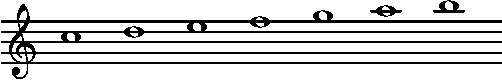
\includegraphics[width=\columnwidth]{c-maj-crop.pdf}
  \begin{tabularx}{\columnwidth}{ YYYYZ }
    &&$ \mathlarger{\mathlarger{\mathlarger{\mathlarger{\mathlarger{\mathlarger\Downarrow}}}}} $ & $A\langle -1,4 \rangle$&
    \end{tabularx}
  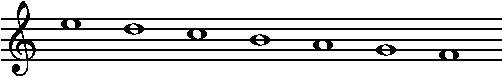
\includegraphics[width=\columnwidth]{e-mod-crop.pdf}
  \caption{L'image de la gamme de \writechord{C} majeur par $A\langle -1,4 \rangle$ est un mode de \writechord{E} }
\end{figure}

Lorsque $\mu = -1$, les transformations $A \langle -1,\tau\rangle : n\mapsto -n + \tau$ permettent de passer d'une gamme majeure à un mode de \writechord{E} et réciproquement. La Figure \ref{fig:inversion} illustre la manière dont l'accord de \writechord{Cma} majeur \writechord{C}$_5$, \writechord{E}$_5$, \writechord{G}$_5$ est transformé par $A\langle -1,4 \rangle$ en l'accord de \writechord{A} mineur  \writechord{A}$_4$, \writechord{C}$_5$, \writechord{E}$_5$, mais aussi envoie l'accord de \writechord{A} mineur \writechord{A}$_4$, \writechord{C}$_5$, \writechord{E}$_5$ sur l'accord de \writechord{Cma} majeur  \writechord{C}$_5$, \writechord{E}$_5$, \writechord{G}$_5$. Comme les transformations affines préservent les classes de hauteur, on peut affirmer plus généralement que $A \langle -1,4\rangle$ envoie \writechord{Cma}  sur \writechord{Ami}   et \writechord{Ami} sur \writechord{Cma}. 

Remarquons de plus que si nous changeons l'ancre, par exemple en choisissant $\alpha = \writechord{G}_4$, l'image de l'accord de \writechord{G} majeur par $A\langle-1,4 \rangle$ sera \writechord{E} mineur. La table \ref{tab:triadesA-14} explicite les images des accords de la gamme de \writechord{Cma} par $A\langle -1,4 \rangle$ lorsque $\alpha = \writechord{C}$ et des accords de la gamme de $G$ majeur lorsque l'on change l'ancre pour $\alpha = \writechord{G}$.


\begin{table}[htbp]
  
  \centering % instead of \begin{center}
  \begin{tabular}{cccccccc}
      \writechord{Cma} & $\mapsto$ & \writechord{Ami} & & & \writechord{Gma} & $\mapsto$ & \writechord{Emi}\\
      \writechord{Dmi} & $\mapsto$ & \writechord{Gma} & & & \writechord{Ami} & $\mapsto$ & \writechord{Dma}\\
      \writechord{Emi} & $\mapsto$ & \writechord{Fma} & & & \writechord{Bmi} & $\mapsto$ & \writechord{Cma}\\
      \writechord{Fma} & $\mapsto$ & \writechord{Emi} & & & \writechord{Cma} & $\mapsto$ & \writechord{Bmi}\\
      \writechord{Gma} & $\mapsto$ & \writechord{Dmi} & & & \writechord{Dma} & $\mapsto$ & \writechord{Ami}\\
      \writechord{Ami} & $\mapsto$ & \writechord{Cma} & & & \writechord{Emi} & $\mapsto$ & \writechord{Gma}\\
      \writechord{Bo} & $\mapsto$ & \writechord{Bo} & & & \writechord{F#o} & $\mapsto$ & \writechord{F#o}
  \end{tabular}
  \caption{Images des accords de la gamme de \writechord{Cma} majeur par $A\langle -1, 4 \rangle$ pour $\alpha = \writechord{C}$ (à gauche) et de la gamme de \writechord{Gma} majeur pour $\alpha = \writechord{G}$ (à droite)} 
  \label{tab:triadesA-14}
\end{table}

Ainsi, en se basant sur l'image de l'accord majeur dont la tonique correspond à l'ancre, nous pouvons associer les transformations affines pour lesquelle $\mu = 1$ ou $\mu=-1$ au degré de l'image de cet accord dans la gamme. Par exemple, $A\langle -1,4 \rangle$ peut être associée au degré \writechord{vi} car elle associe le sixième degré mineur à  l'accord majeur dont la tonique est l'ancre (\writechord{Ami} pour \writechord{Cma}, \writechord{Emi} pour \writechord{Gma}, \dots). On obtient ainsi une notation plus intuitive que la notation mathématique, dont la table \ref{tab:degrees} donne un aperçu. 


\begin{table}[htbp]
  \centering
  \rowcolors{2}{gray!25}{white}
  \begin{tabular}{ccc}
    \rowcolor{gray!50}
    Degré & Transformation affine\\
    \writechord{I} & $A\langle ~~1, ~~0\rangle$\\
    \writechord{ii} &  $A\langle -1, ~~8 \rangle$\\
    \writechord{iii} &  $A\langle -1, -1 \rangle$\\
    \writechord{IV} &  $A\langle ~~1,~~ 5 \rangle$\\
    \writechord{V} &  $A\langle ~~ 1, ~~7 \rangle$\\
    \writechord{vi}& $A\langle -1, ~~4\rangle$\\
    \writechord{vii} & $A\langle -1, ~~3 \rangle$\\
  \end{tabular}
  \caption{ Correspondances entre triades d'une gamme majeure et transformations de gamme\label{tab:degrees} } 
\end{table}







De manière générale, les inversions affines se comportent moins bien sur les modes non naturels. Par exemple, $A\langle -1, 4\rangle (\writechord{G\sharp}) = \writechord{G\sharp}$ donc l'image de la gamme de \writechord{Ami}   harmonique par $A\langle -1, 4\rangle$ contient les notes \writechord{C}, \writechord{D}, \writechord{E}, \writechord{F}, \writechord{G}, \writechord{G\sharp}, \writechord{B}, ce qui ne correspond pas à un mode standard de la musique tonale. C'est une des faiblesses des transformations affines.






